
On cherche à comparer deux milieux de terrain de l'équipe de France de football. Pour cela, on utilise le diagramme en toile d'araignée ci-dessous.

\begin{center}
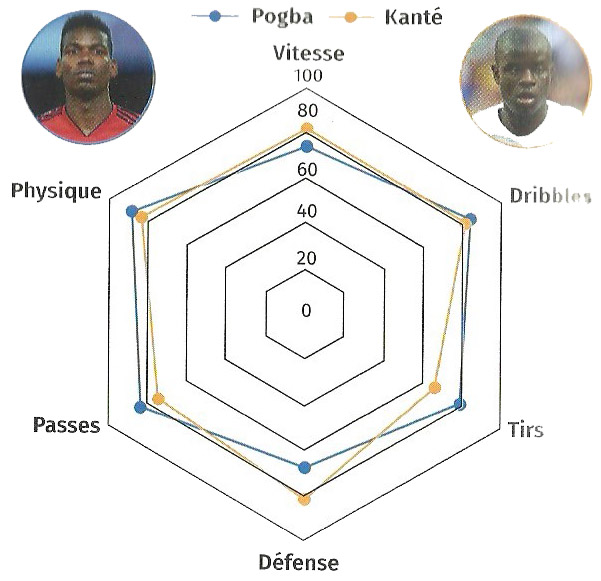
\includegraphics[scale=0.8]{stat-31.jpg}
\end{center}


\begin{enumerate}
\item Donner les domaines sur lesquels les joueurs sont comparés.
\item Sur combien les joueurs sont-ils notés ?
\item Dans quels domaines Pogba est-il plus meilleur que Kanté ?
\item Donner un encadrement de la note de Physique de Kanté.
\item Réaliser une comparaison des deux joueurs en utilisant la médiane approximative et l'écart interquartile de la série donnée par domaine.
\end{enumerate} 